\documentclass[12pt,aspectratio=1610]{beamer}
\RequirePackage{
    amsmath,
    amssymb,
    calc,
    cancel,
    booktabs,
    color,
    siunitx,
    tikz,
    wrapfig,
    array,
    leftidx,
    float,
    etoolbox,
    fancyhdr,
    longtable,
    hyperref,
    ltcaption,
    ulem,
    wasysym,
    accents,
    listings,
    tabularx,
}

\hypersetup{
    hidelinks,
    breaklinks              = true,
}

\usepackage[final]{pdfpages}
\usepackage[many]{tcolorbox}

\RenewDocumentCommand{\vec}{m}{\mathbf{#1}}

\makeatletter
    \def\new@mathgroup{\alloc@8\mathgroup\mathchardef\@cclvi}
    \patchcmd{\document@select@group}{\sixt@@n}{\@cclvi}{}{}
    \patchcmd{\select@group}{\sixt@@n}{\@cclvi}{}{}
\makeatother

\RequirePackage{mathspec}                                   % includes fontspec
\RequirePackage{polyglossia}                                % multi-language support
\RequirePackage{xunicode}
\setdefaultlanguage{slovak}

% Setup fonts -- see fontspec/mathspec documentation.
\defaultfontfeatures{
    Mapping         = tex-text,
    Scale           = MatchLowercase,
    Ligatures       = TeX
}


\NewDocumentCommand{\labelmath}{m +m}{%
    \begin{equation}%
        #2%
        \label{#1}%
    \end{equation}%
}

\NewDocumentCommand{\labelalign}{m +m}{%
    \begin{align}%
        #2%
        \label{#1}%
    \end{align}%
}

\linespread{1.0}
\setlength{\parindent}{0cm}
\setlength{\parskip}{6pt}
\setlength{\abovedisplayskip}{0mm}
\setlength{\belowdisplayskip}{0mm}
\setlength{\abovedisplayshortskip}{0mm}
\setlength{\belowdisplayshortskip}{0mm}
\setlength{\itemindent}{0pt}
\setlength{\textfloatsep}{0mm}
\setlength{\tabcolsep}{3mm}
\setlength{\LTcapwidth}{0.8\textwidth}
\renewcommand{\arraystretch}{1.2}

\setcounter{secnumdepth}{2}

/home/kvik/dgs/core/tex/math.tex
\DeclareSIUnit\au{AU}
\DeclareSIUnit\pixel{px}
\DeclareSIUnit\lightyear{ly}
\DeclareSIUnit\parsec{pc}
\DeclareSIUnit\earthmass{M_{\earth}}
\DeclareSIUnit\speedoflight{c}
\DeclareSIUnit\foe{foe}
\DeclareSIUnit\year{yr}
\DeclareSIUnit\eur{€}
\DeclareSIUnit\solarmass{M_{\astrosun}}
\DeclareSIUnit\solarluminosity{L_{\astrosun}}
\DeclareSIUnit{\byte}{B}




\linespread{1.0}
\setlength{\parindent}{0cm}
\setlength{\parskip}{6pt}
\setlength{\abovedisplayskip}{0mm}
\setlength{\belowdisplayskip}{0mm}
\setlength{\abovedisplayshortskip}{0mm}
\setlength{\belowdisplayshortskip}{0mm}
\setlength{\itemindent}{0pt}
\setlength{\textfloatsep}{0mm}
\setlength{\tabcolsep}{3mm}
\renewcommand{\arraystretch}{1.2}

\setcounter{secnumdepth}{0}

\NewDocumentCommand{\fspicture}{m O{W} O{black}}{
    {
        \setbeamertemplate{navigation symbols}{}
        \setbeamercolor{background canvas}{bg = #3}
        \begin{frame}[plain]
            \begin{tikzpicture}[remember picture, overlay]
                \node[at=(current page.center)] {
                    \ifstrequal{H}{#2}{                                  
                        \includegraphics[height=\paperheight]{#1}%
                    }{%
                        \includegraphics[width=\paperwidth]{#1}%
                    }
                };
            \end{tikzpicture}
        \end{frame}
    }
}

\NewDocumentCommand{\frejm}{m +m}{
    \begin{frame}
        \frametitle{#1}
        #2
    \end{frame}
}

\NewDocumentCommand{\fragfrejm}{m +m}{
    \begin{frame}[fragile]
        \frametitle{#1}
        #2
    \end{frame}
}

\defbeamertemplate{description item}{align center}{\hfill\insertdescriptionitem\hfill}
\definecolor{desc}{rgb}{0.66, 0, 0}
\definecolor{citem}{rgb}{0.72, 0, 0}
\definecolor{csitem}{rgb}{0.90, 0, 0}
\definecolor{cssitem}{rgb}{1, 0.1, 0.1}
\definecolor{qprimarybg}{rgb}{0.95, 0.95, 0.95}
\definecolor{check}{rgb}{0, 0.8, 0}
\definecolor{coded}{rgb}{0.9, 0.9, 0.9}
\definecolor{todo}{rgb}{1.0, 0.3, 0.3}
\definecolor{model}{rgb}{0.75, 0, 0}

\setbeamertemplate{navigation symbols}{}
\newfontfamily{\semibold}{Segoe UI Semibold}
\RenewDocumentCommand{\emph}{m}{{\semibold#1}}
\NewDocumentCommand{\code}{m}{\textcolor{desc}{\texttt{#1}}}
\NewDocumentCommand{\model}{m}{\colorbox{coded}{\textcolor{model}{\texttt{#1}}}}
\NewDocumentCommand{\todo}{m}{\colorbox{todo}{#1}}

\mode<presentation> {
    \usetheme{Szeged}
    \usecolortheme{beaver}
    
    \usefonttheme{professionalfonts}
    \setallmainfonts{Minion Pro}
    \setmathrm{Minion Pro}
    
    \setsansfont{Segoe UI}
    \setmonofont{Consolas}
    \setbeamercolor*{enumerate item}{fg = citem}
    \setbeamercolor*{enumerate subitem}{fg = csitem}
    \setbeamercolor*{enumerate subsubitem}{fg = cssitem}
    \setbeamercolor*{description item}{fg = desc}
    \setbeamercolor*{itemize item}{fg = citem}
    \setbeamercolor*{itemize subitem}{fg = csitem}
    \setbeamercolor*{itemize subsubitem}{fg = cssitem}
    \setbeamercolor*{palette primary}{fg = red, bg = qprimarybg}
}

\newcommand<>\highlightbox[2]{%
    \alt#3{\makebox[\dimexpr\width-2\fboxsep]{\colorbox{#1}{#2}}}{#2}%
}

\AtBeginSection[]{
    \subsection{\insertsection}
    \begin{frame}
        \vfill
        \centering
        \begin{beamercolorbox}[sep = 18pt, center, shadow = true, rounded = true]{title}
            \usebeamerfont{title}\insertsectionhead%
            \vfill
        \end{beamercolorbox}
        \vfill
    \end{frame}
}

\makeatletter
% Render percent sign with nice font, not ugly Computer modern
    \mathcode`\%="7025

% Fixes mathspec bug -- URL numbers are rendered with wrong font
    \ernewcommand\eu@MathPunctuation@symfont{Latin:m:n}
    \DeclareMathSymbol{,}{\mathpunct}{\eu@MathPunctuation@symfont}{`,}
    \DeclareMathSymbol{?}{\mathpunct}{\eu@MathPunctuation@symfont}{`?}
    \DeclareMathSymbol{.}{\mathord}{\eu@MathPunctuation@symfont}{`.}
    \DeclareMathSymbol{<}{\mathrel}{\eu@MathPunctuation@symfont}{`<}
    \DeclareMathSymbol{>}{\mathrel}{\eu@MathPunctuation@symfont}{`>}
    \DeclareMathSymbol{/}{\mathord}{\eu@MathPunctuation@symfont}{`/}
    \DeclareMathSymbol{;}{\mathpunct}{\eu@MathPunctuation@symfont}{`;}
    \DeclareMathSymbol{(}{\mathopen}{\eu@DigitsArabic@symfont}{`(}
    \DeclareMathSymbol{)}{\mathclose}{\eu@DigitsArabic@symfont}{`)}
    \XeTeXDeclareMathSymbol{^^^^2026}{\mathinner}{\eu@MathPunctuation@symfont}{"2026}[\mathellipsis]
    \DeclareMathSymbol{0}{\mathalpha}{\eu@DigitsArabic@symfont}{`0}
    \DeclareMathSymbol{1}{\mathalpha}{\eu@DigitsArabic@symfont}{`1}
    \DeclareMathSymbol{2}{\mathalpha}{\eu@DigitsArabic@symfont}{`2}
    \DeclareMathSymbol{3}{\mathalpha}{\eu@DigitsArabic@symfont}{`3}
    \DeclareMathSymbol{4}{\mathalpha}{\eu@DigitsArabic@symfont}{`4}
    \DeclareMathSymbol{5}{\mathalpha}{\eu@DigitsArabic@symfont}{`5}
    \DeclareMathSymbol{6}{\mathalpha}{\eu@DigitsArabic@symfont}{`6}
    \DeclareMathSymbol{7}{\mathalpha}{\eu@DigitsArabic@symfont}{`7}
    \DeclareMathSymbol{8}{\mathalpha}{\eu@DigitsArabic@symfont}{`8}
    \DeclareMathSymbol{9}{\mathalpha}{\eu@DigitsArabic@symfont}{`9}
\makeatother


\title{Spatial density and model of meteoroid population}
\subtitle{PhD thesis project defence}
\author{\small \emph{Martin Baláž}}
\institute{DAPEM FMPH, Comenius University}
\date{2020--05--18}

\begin{document}
    {
        \usebackgroundtemplate{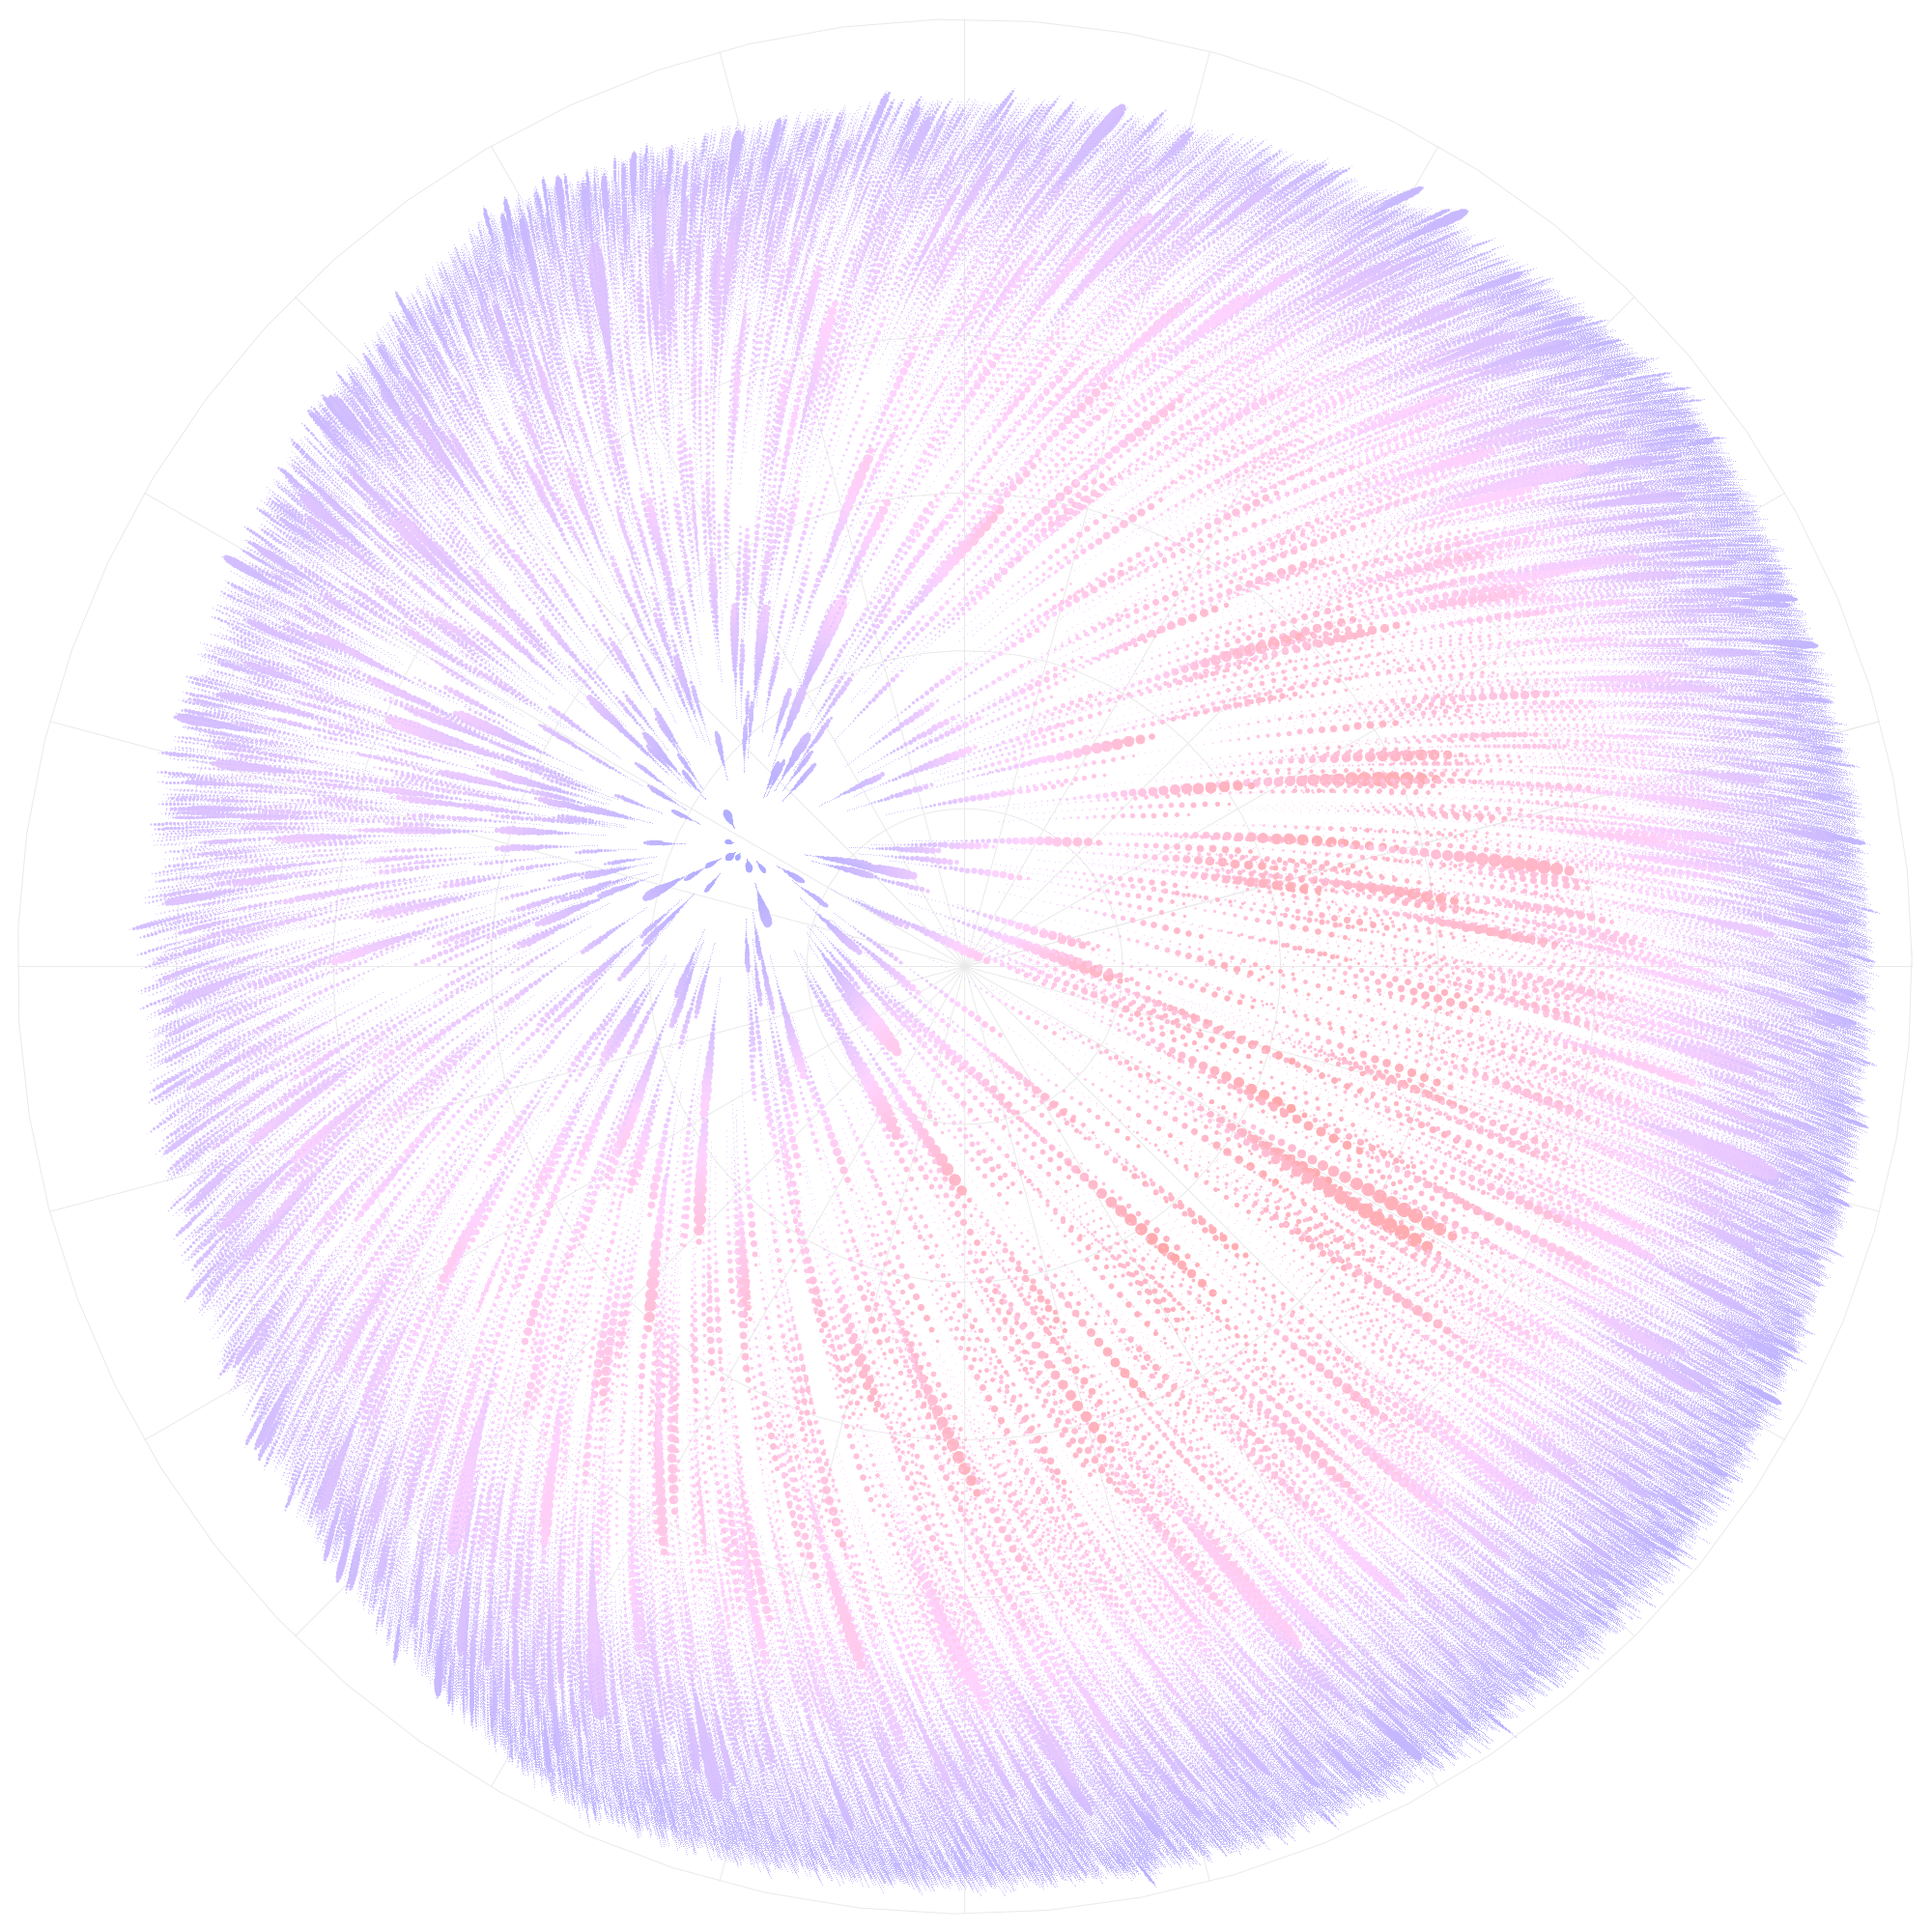
\includegraphics[width=\paperwidth]{pictures/fireworks-i.png}}
        \begin{frame}
            \titlepage
        \end{frame}
    }
    \section{Overview}
        \frejm{Objective}{
            Develop a \emph{model} of meteoroid distribution
            \pause
            \begin{itemize}
                \item we have
                \begin{itemize}
                    \item observations by AMOS
                    \item simulation toolkit ASMODEUS
                \end{itemize}
                \pause
                \item we want to
                \begin{itemize}
                    \item describe \emph{distributions} of meteor[oid]s
                    \item ...and of their properties
                \end{itemize}
            \end{itemize}
        }

        %\fspicture{pictures/overview.png}[H]
        %\fspicture{pictures/mapAMOS.png}[H]
        %\fspicture{pictures/KNM.jpg}[H]
        %\fspicture{pictures/Perseids.jpg}[H]

        %\fspicture{pictures/streaks.png}[H]
        %\fspicture{pictures/dots.png}[H]

    \section{Analysis}
        \frejm{Meteors and meteoroids}{
            \begin{columns}
                \begin{column}{0.5\textwidth}
                    Problems:
                    \begin{itemize}
                        \pause
                        \item meteoroids
                        \begin{itemize}
                            \item cannot be \emph{observed} directly
                            \item extreme selection bias
                        \end{itemize}
                    \end{itemize}
                    \pause
                    \begin{itemize}
                        \item meteors
                        \begin{itemize}
                            \item are \emph{transient} phenomena
                            \item properties dependent on observer
                            \item strong selection bias
                        \end{itemize}
                    \end{itemize}
                \end{column}
                \pause
                \begin{column}{0.5\textwidth}
                    Solution: build \emph{two models}
                    \pause
                    \begin{itemize}
                        \item \emph{observational model} for meteors
                        \item \emph{orbital model} for meteoroids
                    \end{itemize}
                    \vfill
                \end{column}
            \end{columns}
        }

        \frejm{How?}{
            We have \emph{discrete} events
            \begin{itemize}
                \item treat meteors as \emph{random samples}
                \item from some continuous $N$-dimensional \emph{distribution}
            \end{itemize}
            \pause
            \begin{itemize}
                \item How do we \emph{describe} these samples?
                \item How do we obtain a distribution from samples?
            \end{itemize}
        }

        \frejm{Observational model}{
            Estimates the distribution of meteors in the sky
            \pause
            \begin{itemize}
                \item<2-> time (1)
                \item\only<3>{position}\only<4->{\sout{position}}
                \item<4-> radiant (2+1)
                \item<5-> magnitude spectrum (1)
            \end{itemize}
            $$
                \only<5->{
                    \mathcal{A}(t, \vec{v}, m) \equiv \mathcal{A}(t, \delta_\mathrm{R}, \alpha_\mathrm{R}, v_\infty, m).
                }
            $$
        }

        \frejm{Orbital model}{
            Observational model tells \emph{when} and \emph{what}...
            \pause
            but does not tell \emph{why}
            \pause
            \begin{itemize}
                \item time (1)
                \item position (3)
                \item velocity (3)
                \item mass spectrum (1)
            \end{itemize}
            \pause
            $$
                \mathcal{M}_{\mathrm{rv}}(t, \vec{r}, \vec{v}, \mu) \quad\text{or}\quad
                \mathcal{M}_{\mathrm{oe}}(t, a, e, i, \omega, \Omega, T, \mu)
            $$
            \pause
            or better
            $$
                \mathcal{M}_{\mathrm{rv}}(t, \vec{r}, \vec{v}, \log \mu) \quad\text{or}\quad
                \mathcal{M}_{\mathrm{oe}}(t, 1/a, e, i, \omega, \Omega, T, \log \mu)
            $$
        }


    \setbeamersize{description width = 5mm}

    \section{Methods}
        \frejm{Histograms}{
            Simple, robust method

            \begin{itemize}
                \item does not produce useful predictions
                \item loses correlation between properties
            \end{itemize}
        }

        \frejm{Kernel density estimation}{
            We can generalize histograms to be continuous

            \pause
            \begin{itemize}
                \item basic idea
                \begin{itemize}
                    \item replace every observation by a \emph{kernel}
                    \item \emph{sum} the kernels
                    \pause
                    \item this is our estimate of the distribution
                \end{itemize}
                \item we can sample it to obtain realistic synthetic meteors
            \end{itemize}
        }

        \fspicture{pictures/shift.png}[][white]
        \fspicture{pictures/kde.png}[][white]

        \frejm{One dimension}{
            \begin{itemize}
                \item we need to set the \emph{bandwidth} of the kernel
                \pause
                \item similar to bin width in histograms
            \end{itemize}
            $$
                \Hat[-1pt]{f}(\vec{x}) = \frac{1}{nh} \Sum[i = 1][n]{K\left(\frac{x - x_i}{h}\right)}
            $$
        }

        \frejm{Goodness of fit}{
            If we know the true distribution, we can design a metric
            \begin{itemize}
                \item \emph{MISE}
            \end{itemize}
            $$
                \mathrm{MISE}(\Hat[-1pt]{f}(x), f\,(x)) = \Int[\mathbb{R}]{\left(\Hat[-1pt]{f}(x) - f\,(x) \right)^2}{x}
            $$

            \pause
            \begin{itemize}
                \item cross-validation, leave-$p$-out
            \end{itemize}
        }

        \frejm{Multiple dimensions}{
            KDE easily \emph{generalizes} to multivariate functions
            $$
                \Hat[-1pt]{f}(\vec{x}) = \frac{1}{n h} \Sum[i = 1][n]{K\left(\frac{\vec{x} - \vec{x}_i}{h}\right)}
            $$
            \pause
            \begin{itemize}
                \item but the variables may be \emph{correlated}
                \item we need to find the \emph{correlation matrix} $\vec{H}$
                \begin{itemize}
                    \item symmetric, positive-definite
                \end{itemize}
            \end{itemize}
            \pause
            $$
                \Hat[-1pt]{f}(\vec{x}) = \frac{1}{n \Abs{\vec{H}}} \Sum[i = 1][n]{K\left(\vec{H}^{-1}\left(\vec{x} - \vec{x}_i\right)\right)}
            $$
        }

        %\fspicture{pictures/shift.png}[][white]
        %\fspicture{pictures/kde.png}[][white]

        %\frejm{Convolution}{
        %    KDE can be defined as a convolution
        %    $$
        %        \Hat[-1pt]{f}(\vec{x}) = \frac{1}{n \Abs{\vec{H}}} \left(\vec{H}^{-1} K * \left(\Sum[i = 1][n]{\delta\left(\vec{x} - \vec{x}_i\right)\right)} \right)
        %    $$
        %    \pause
        %    \begin{itemize}
        %        \item mathematically beautiful
        %        \item but not very practical
        %    \end{itemize}
        %}

        \frejm{Adaptive KDE}{
            Bandwidth need not be constant
            \begin{itemize}
                \item it might be beneficial to vary bandwidth
                \begin{itemize}
                    \item different points use different $\vec{H}$ or $h$
                \end{itemize}
                \pause
                \item generally
                \begin{itemize}
                    \item narrow bandwidth where data are \emph{abundant}
                    \item wide bandwidth where data are \emph{sparse}
                \end{itemize}
            \end{itemize}
        }

    \section{Algorithm}
        \frejm{Overview}{
            \begin{itemize}
                \item we want to find PDFs for \emph{meteors} and \emph{meteoroids}
                \pause
                \begin{enumerate}
                    \item take data from AMOS
                    \item correct for selection bias
                    \item design a suitable $\vec{H}$
                    \item run the KDE for meteors
                    \item find consistent orbital model
                \end{enumerate}
            \end{itemize}
        }

        \fspicture{pictures/model.png}[][white]

        \frejm{Curse of dimensionality}{
            $N$-volume of parameter space increases exponentially
            \begin{itemize}
                \item the space is \emph{vast}
                \pause
                \item $\ang{360} \times \ang{180} \times \num{8766} \times \num{50} \times \num{50} \approx \num{1.42e12}$
                \pause
                \item we should use a \emph{mesh} instead of a \emph{grid}
                \item almost all of it is ``in the corner''
                \item distance metrics are not very useful
            \end{itemize}
        }

    \section{Summary}
        \frejm{Summary}{
            \begin{itemize}
                \item we want to build model/prediction of meteor activity
                \item using KDE extrapolation of AMOS data
                \item separate (but related) models for \emph{meteors} and \emph{meteoroids}
            \end{itemize}
        }

        \frejm{References}{
            \begin{itemize}
                \item \textbf{Hwang, J.-N. -- Lay, S.-R. and Lippman, A.}:
                    Nonparametric multivariate density estimation: a case study.
                    IEEE Transactions on Signal Processing 42, 1994.
                \item \textbf{Vida, D. -- Brown, P. -- Campbell-Brown, M.}:
                    Modeling the measurement accuracy of pre-atmosphere velocities of meteoroids. MNRAS 479, 2018
                \item \textbf{Vida, D. -- Brown, P. -- Campbell-Brown, M.}:
                    Generating realistic synthetic meteoroid orbits. Icarus 296, 2017.
                \item Wikipedia, user \textbf{Drleft}:
                    Synthetic data 2D histograms, 2010.\\ \small
                    \url{https://en.wikipedia.org/wiki/File:Synthetic_data_2D_histograms.png}
                \item Wikipedia, user \textbf{Drleft}:
                    Synthetic data 2D KDE, 2010.\\ \small
                    \url{https://en.wikipedia.org/wiki/File:Synthetic_data_2D_KDE.png}
            \end{itemize}
        }

    \section{Questions}{
        \frejm{1. otázka}{
            \textit{Prečo je “t” v “the” v 1. riadku časti “Zenithal hourly rate” na str. 26 v hranatých zátvorkách?}
            \pause
            \par
            Je to citát, pôvodne to bolo veľkým.
        }

        \frejm{2. otázka}{
            \textit{Môže ašpirant načrtnúť odvodenie vzťahu (2.2.9), ktorý je uvedený na str. 33? Ako bol získaný
                výraz $\left(s - 1\right)\mu_{\mathrm{min}}^{s-1}$ vo význame konštanty úmernosti?
                Nenulový výraz na pravej strane vzťahu má rozmer reciprokej hmotnosti. Je to správne?
            }
            \pause
            \par
            Je to prirodzený spôsob, ako získať PDF úmernú $\mu^{-s}$.
            Aby nedivergovala, musí byť zdola ohraničená $\mu_{\mathrm{min}}$.
            Zároveň musí byť normovaná,
            $$
                \Int[0][\infty]{\varrho(\mu)}{\mu} = 1
            $$
            Tieto podmienky spĺňa jedine uvedené riešenie.
        }

        \frejm{3. otázka}{
            \textit{V 3. odstavci na str. 35 je uvedené, že každá častica, ktorá pretne účinný prierez Zeme, je
                označená ako “zachytená” a potom ďalej vyšetrovaná (zrejme kvôli predpovedaniu vlastností
                príslušného roja. Myslí ašpirant na tomto mieste prelet účinným prierezom zemského telesa len ak
                sa tam Zem v danom čase nachádza? Alebo má na mysli prelet okolo zemskej dráhy vo vzdialenosti
                rovnej alebo menšej ako je polomer Zeme?
            }
            \pause
            \par
            Iba v zodpovedajúcom čase, keď sa tam Zem skutočne nachádza.

            \pause
            \textit{V uvedenom odstavci ďalej je potom uvedené, že polomer simulovanej Zeme je umelo zväčšený
                niekoľko krát, aby bolo zachytených viac meteorov. O aké zväčšenie sa, číselne, jedná?}
            \pause
            \par
            V súčasnosti neviem zodpovedať, odhadujem rádovo 5. Musí sa zachovať podmienka konštantnosti hustoty.
        }

        \frejm{4. otázka}{
            \textit{V opise simulácie v kap. 2.3.1 na str. 34 a 35 nie je uvedené, akým smerom v čase (či do
                budúcnosti alebo do minulosti) a počas akej dlhej doby je pohyb častíc sledovaný numerickou
                integráciou. A či sú alebo nie sú brané do úvahy aj negravitačné sily, ak áno, aké. Môže ašpirant túto
                informáciu doplniť?
            }
            \pause
            \par
            Z minulosti smerom do súčasnosti, na základe predchádzajúcich známych modelov.

            Negravitačné pôsobenie musíme uvažovať (ejekčné rýchlosti, tlak žiarenia, Poynting-Robertsonov efekt).
        }

        \frejm{5. otázka}{
            \textit{Predposledný odstavec na str. 39 začínajúci “To simplify...” je nezrozumiteľný. Môže ašpirant
                uviesť príklad tam spomínanej diagonálnej matice s odlišnou metrikou ako má kovariantná matica?
                A vysvetliť, prečo sú sférické súradnice problematické?
            }
            \pause
            \par
            "Metrika" sa vzťahuje na celý algoritmus, nie na maticu. Diagonálna matica spôsobí, že pre rôzne
            veličiny bude rôzny bandwidth, ale bez korelácií.

            Pri sférickej metrike sa tvar kernelu nutne mení (príklad).
        }

\end{document}
